%%
%% This is file `sample-manuscript.tex',
%% generated with the docstrip utility.
%%
%% The original source files were:
%%
%% samples.dtx  (with options: `manuscript')
%% 
%% IMPORTANT NOTICE:
%% 
%% For the copyright see the source file.
%% 
%% Any modified versions of this file must be renamed
%% with new filenames distinct from sample-manuscript.tex.
%% 
%% For distribution of the original source see the terms
%% for copying and modification in the file samples.dtx.
%% 
%% This generated file may be distributed as long as the
%% original source files, as listed above, are part of the
%% same distribution. (The sources need not necessarily be
%% in the same archive or directory.)
%%
%% The first command in your LaTeX source must be the \documentclass command.
\documentclass[manuscript,screen]{acmart}

%%
%% \BibTeX command to typeset BibTeX logo in the docs
\AtBeginDocument{%
  \providecommand\BibTeX{{%
    \normalfont B\kern-0.5em{\scshape i\kern-0.25em b}\kern-0.8em\TeX}}}

%% Rights management information.  This information is sent to you
%% when you complete the rights form.  These commands have SAMPLE
%% values in them; it is your responsibility as an author to replace
%% the commands and values with those provided to you when you
%% complete the rights form.
\setcopyright{acmcopyright}
\copyrightyear{2021}
\acmYear{2021}
%\acmDOI{10.1145/1122445.1122456}

%% These commands are for a PROCEEDINGS abstract or paper.
\acmConference [RecSys'21] %{15th ACM Conference on Recommender Systems} {27th September-1st October 2021}
{Amsterdam, Netherlands}
{15th ACM Conference on Recommender Systems, Amsterdam, Netherlands, 27th September-1st October 2021}

\acmBooktitle{15th ACM Conference on Recommender Systems,  Amsterdam, Netherlands, 27th September-1st October 2021}

\acmPrice{15.00}
\acmISBN{978-1-4503-XXXX-X/18/06}


%%
%% Submission ID.
%% Use this when submitting an article to a sponsored event. You'll
%% receive a unique submission ID from the organizers
%% of the event, and this ID should be used as the parameter to this command.
%%\acmSubmissionID{123-A56-BU3}

%%
%% The majority of ACM publications use numbered citations and
%% references.  The command \citestyle{authoryear} switches to the
%% "author year" style.
%%
%% If you are preparing content for an event
%% sponsored by ACM SIGGRAPH, you must use the "author year" style of
%% citations and references.
%% Uncommenting
%% the next command will enable that style.
%%\citestyle{acmauthoryear}

%%
%% end of the preamble, start of the body of the document source.
\begin{document}

%%
%% The "title" command has an optional parameter,
%% allowing the author to define a "short title" to be used in page headers.
\title{Impact of Variations of Similarity and Prediction Techniques on User-based and Item-based Collaborative Filtering Recommendations}

%%
%% The "author" command and its associated commands are used to define
%% the authors and their affiliations.
%% Of note is the shared affiliation of the first two authors, and the
%% "authornote" and "authornotemark" commands
%% used to denote shared contribution to the research.

\author{First Lastname1}
\affiliation{%
  \institution{Davidson College}
  \streetaddress{102 N Main Street}
  \city{ Davidson}
  \state{ North Carolina}
  \postcode{ 28036}
  \country{USA} }
\email{jadoe@davidson.edu}

\author{First Lastname2}
\affiliation{%
  \institution{Davidson College}
  \streetaddress{102 N Main Street}
  \city{ Davidson}
  \state{ North Carolina}
  \postcode{ 28036}
    \country{USA} } 
\email{jodoe@davidson.edu}

\author{First Lastname3}
\affiliation{%
  \institution{Davidson College}
  \streetaddress{102 N Main Street}
  \city{ Davidson}
  \state{ North Carolina}
  \postcode{ 28036}
    \country{USA} } 
\email{jadoe@davidson.edu}

\author{First Lastname4}
\affiliation{%
  \institution{Davidson College}
  \streetaddress{102 N Main Street}
  \city{ Davidson}
  \state{ North Carolina}
  \postcode{ 28036}
    \country{USA} } 
\email{jodoe@davidson.edu}

%%
%% By default, the full list of authors will be used in the page
%% headers. Often, this list is too long, and will overlap
%% other information printed in the page headers. This command allows
%% the author to define a more concise list
%% of authors' names for this purpose.
\renewcommand{\shortauthors}{NAMES: One, Two, Three, Four}

%%
%% The abstract is a short summary of the work to be presented in the
%% article.
\begin{abstract}
Recommender Systems provide users with product/service recommendations in order to save time and effort maneuvering through the plethora of choices available. This work reviews various Similarity and Prediction Techniques used in the generation of Collaborative Filtering User-based and Item-based Recommendations.
\end{abstract}

%%
%% The code below is generated by the tool at http://dl.acm.org/ccs.cfm.
%% Please copy and paste the code instead of the example below.
%%
%\begin{CCSXML}
%<ccs2012>
% <concept>
%  <concept_id>10010520.10010553.10010562</concept_id>
%  <concept_desc>Computer systems organization~Embedded systems</concept_desc>
%  <concept_significance>500</concept_significance>
% </concept>
% <concept>
%  <concept_id>10010520.10010575.10010755</concept_id>
%  <concept_desc>Computer systems organization~Redundancy</concept_desc>
%  <concept_significance>300</concept_significance>
% </concept>
% <concept>
%  <concept_id>10010520.10010553.10010554</concept_id>
%  <concept_desc>Computer systems organization~Robotics</concept_desc>
%  <concept_significance>100</concept_significance>
% </concept>
% <concept>
%  <concept_id>10003033.10003083.10003095</concept_id>
%  <concept_desc>Networks~Network reliability</concept_desc>
%  <concept_significance>100</concept_significance>
% </concept>
%</ccs2012>
%\end{CCSXML}
%
%\ccsdesc[500]{Computer systems organization~Embedded systems}
%\ccsdesc[300]{Computer systems organization~Redundancy}
%\ccsdesc{Computer systems organization~Robotics}
%\ccsdesc[100]{Networks~Network reliability}

%%
%% Keywords. The author(s) should pick words that accurately describe
%% the work being presented. Separate the keywords with commas.
\keywords{Recommender Systems, Collaborative Filtering, Similarity and Prediction techniques}


%%
%% This command processes the author and affiliation and title
%% information and builds the first part of the formatted document.
\maketitle

\section{Introduction}
Introduce your work effort here. Explain the motivation for undertaking this work and the importance to the Recommender System field. Include a brief discussion of research questions to be pursued/answered in this study. Indicate any novel approaches.

\section{Related Work}
This section presents the prior work that has been conducted in this area of research. Use citations and the accomplishments of the prior work.

\section{Thesis}
This section explains the research that will be performed in this work (WHAT), 
details of the motivation behind this effort (WHY), 
a discussion of the Hypotheses that will be tested (EXPECTED RESULTS),
 and a brief description of how the research effort will be conducted (HOW). 
 Use formulae and/or equations to detail the math behind this effort.

\section{Experimental Design}
This section lays out the assumptions and variations of the study. What datsaets were used. What variables will be varied and the extent to which they will be varied. Etc.

\textbf{Experimental Design/Variations Requirements (~ 36 variations total): }
\begin {itemize}
\item Recommender System Algorithms: User-based and Item-based
\item Similarity method: Distance, Pearson (+optional=Spearman or Jaccard or Tanimoto, etc.)
\item Similarity significance weighting: None, n/25, n/50 (+optional= n/75, n/100, or variance weighting)
\item Similarity threshold: >0, >0.3, >0.5 (+optional= >0.1, >0.2, >0.4)
\item Rating prediction normalization: weighted (+optional=deviation-from-mean weighted or  z-score predictions)
\item Datasets: ML-100K (run some variations with critics first for testing; must provide Stats report for ML-100K)
\item Evaluation: LOOCV (+optional=k-fold CV)
\item Metrics: MSE, RMSE, MAE (report all three together)
\item Tests of Hypothesis: (+optional=p-values for pairs of means or ANOVA for multiple means)
\end {itemize}

Note: Any +optional(s) selected will need to run with all other requirements.\\


Code development does not have to be described; neither does computing configuration. I would strongly suggest that you continue to build on the code base we have been developing in class. Your code should be well documented and readable! \textbf{Here are some additional programming that will be required:}
\begin {enumerate} 
\item Extensions to LCVSIM command: 

\begin {itemize}
\item Check for a larger len(prrefs) and name accordingly
\item Have the user enter either User-based or Item-based recommendations. Be sure to set algo to correspond to the input .. algo = getRecommendationsSim or  algo = getRecommendedItems
\item Asking for error metric no longer required since your loo\_cv\_sim() code will calc/print all three at the end of each run.
\item Be sure to run SIM or SIMU commands before executing this command.
\end {itemize}

\item New SIMU command: similar to SIM command except that this reads/writes a User-User similarity matrix. This command will need to call the new calculateSimilarUsers() function described below.

\item New RML(ead ml-100k dataset). Downloaded the ml-100k zip from GroupLens.org, unzip and place the contents into a ``ml-100k'' folder located in the ``data'' folder where the ``critics'' data are stored. Here's some code for RML ..
\begin{verbatim}
        elif file_io == 'RML' or file_io == 'rml':
            print()
            file_dir = 'data/ml-100k/' # path from current directory
            datafile = 'u.data'  # ratngs file
            itemfile = 'u.item'  # movie titles file            
            print ('Reading "%s" dictionary from file' % datafile)
            prefs = from_file_to_dict(path, file_dir+datafile, file_dir+itemfile)
            print('Number of users: %d\nList of users [0:10]:' 
                  % len(prefs), list(prefs.keys())[0:10] ) 
\end{verbatim}

\item Extensions to loo\_cv\_sim() function:

\begin {itemize}
\item Calls the getRecommendationsSim() function for user-based recommendations and getRecommendedItems for item-based recommendations
\item Calc /report MSE, RMSE, and MAE at the end of each run
\item Remove the metric parameter since your code will calc all three.
\end {itemize}

\item New getRecommendationsSim() function: Similar to getRecommendations() function but uses the user-user sim matrix (created by the calculateSimilarUsers() function) to calculate recommendations (much faster, but not as precise perhaps).

\item New calculateSimilarUsers() function: Similar to calculateSimilarItems() function but for users instead of items so no transpose required. This function is called by SIMU. \textbf{Be sure to set n=100 in the parameter list for this function and for calculateSimilarItems() as well!}

\end {enumerate}


\textbf{Additional Requirements:}
\begin {itemize}
 \item Required sections: Abstract, Introduction, Related Work, Thesis, Experimental Design, Results, Discussion, Conclusion, References
  \item Documentation: Use of LaTeX including bib, use ACM template
  \item Figures: Use of Excel/matplotlib/etc., png/jpg/gif/etc.
  \item Code: Python v3 -- Well documented and readable!
  
  \item Moodle Deliverable (zipped file): 
  
  \begin {enumerate} 
  \item Technical paper pdf file
  \item Folder 1: LaTeX tex file, and everything required to generate the pdf document such as bib file (if used), figures, etc.
   \item Folder 2: Code py file(s) with instructions on how to run the program(s)
   \item Folder 3: Data files used/generated
 \end {enumerate}
 
\item Teaming: Teams will be assigned
\item Honor Code: This is a pledged activity. No sharing of work/content between teams is allowed. Do not represent other?s work as your own.
\item Grading Rubric:  Grade reflects the degree to which the criteria below are satisfied: 90-100: All/most, 80-89.99: Many/some, 70-79.99: Few/lacking, 60-69.99: Needs major re-work, below 60: no meaningful content delivered. \textbf{These cutoffs will be further defined for clarity.} High quality optional work will be used to potentially improve the final grade.

  \begin {enumerate} 
\item  Completeness (40\%): Meets requirements and specifications
\item Quality of content (60\%): Clarity of expression (text, formulae, figures, etc.), methodical approach, meaningful content in all required sections, analytical discussion of results
  \end {enumerate}

 \end {itemize}


\section{Results}
Provide text, charts, and tables that indicate/explain the results that were obtained by executing the Experimental Design.

\begin {verbatim}
Descriptive analytics data/Chart for ml-100K:
-- Total number of users, items, ratings
-- Overall average rating, standard dev (all users, all items)
-- Average item rating, standard dev (all users)
-- Average user rating, standard dev (all items)
-- Matrix ratings sparsity
-- Ratings distribution histogram (all users, all items)

Popular items analytics data/Chart for ml-100K: 
-- popular items: most rated (sorted by # ratings)
-- popular items: highest rated (sorted by avg rating)
-- popular items: highest rated items that have 
   at least a "threshold" number of ratings


Results Charts:
Calc MSE, RMSE, and MAE for each run so your don't have to repeat the run just for a different error metric

1. User-based Recommendation, y-axis: MSE, x-axis: simWtg (none, n25, n50)
   Curve1: Pearson+>0sim
   Curve2: Pearson+.3sim
   Curve3: Pearson+.5sim
   Curve4: Distance+>0sim
   Curve5: Distance+.3sim
   Curve6: Distance+.5sim
   
    Variations:
    User/Pearson/NosimWtg/>0sim/Wtgd/ml100k/MSE
    User/Pearson/n25simWtg/>0sim/Wtgd/ml100k/MSE
    User/Pearson/n50simWtg/>0sim/Wtgd/ml100k/MSE
    User/Distance/NosimWtg/>0sim/Wtgd/ml100k/MSE
    User/Distance/n25simWtg/>0sim/Wtgd/ml100k/MSE
    User/Distance/n50simWtg/>0sim/Wtgd/ml100k/MSE
    
    User/Pearson/NosimWtg/.3sim/Wtgd/ml100k/MSE
    User/Pearson/n25simWtg/.3sim/Wtgd/ml100k/MSE
    User/Pearson/n50simWtg/.3sim/Wtgd/ml100k/MSE
    User/Distance/NosimWtg/.3sim/Wtgd/ml100k/MSE
    User/Distance/n25simWtg/.3sim/Wtgd/ml100k/MSE
    User/Distance/n50simWtg/.3sim/Wtgd/ml100k/MSE
    
    User/Pearson/NosimWtg/.5sim/Wtgd/ml100k/MSE
    User/Pearson/n25simWtg/.5sim/Wtgd/ml100k/MSE
    User/Pearson/n50simWtg/.5sim/Wtgd/ml100k/MSE
    User/Distance/NosimWtg/.5sim/Wtgd/ml100k/MSE
    User/Distance/n25simWtg/.5sim/Wtgd/ml100k/MSE
    User/Distance/n50simWtg/.5sim/Wtgd/ml100k/MSE


2. User-based Recommendation, y-axis: RMSE, x-axis: simWtg (none, n25, n50)
       Same as chart 1 but with RMSE.
       Curve1: Pearson+>0sim
       Curve2: Pearson+.3sim
       Curve3: Pearson+.5sim
       Curve4: Distance+>0sim
       Curve5: Distance+.3sim
       Curve6: Distance+.5sim

3. User-based Recommendation, y-axis: MAE, x-axis: simWtg (none, n25, n50)
       Same as chart 1 but with MAE.
       Curve1: Pearson+>0sim
       Curve2: Pearson+.3sim
       Curve3: Pearson+.5sim
       Curve4: Distance+>0sim
       Curve5: Distance+.3sim
       Curve6: Distance+.5sim



4. Item-based Recommendation, y-axis: MSE, x-axis: simWtg (none, n25, n50)
       Curve1: Pearson+>0sim
       Curve2: Pearson+.3sim
       Curve3: Pearson+.5sim
       Curve4: Distance+>0sim
       Curve5: Distance+.3sim
       Curve6: Distance+.5sim

        Variations:
        Item/Pearson/NosimWtg/>0sim/Wtgd/ml100k/MSE
        Item/Pearson/n25simWtg/>0sim/Wtgd/ml100k/MSE
        Item/Pearson/n50simWtg/>0sim/Wtgd/ml100k/MSE
        Item/Distance/NosimWtg/>0sim/Wtgd/ml100k/MSE
        Item/Distance/n25simWtg/>0sim/Wtgd/ml100k/MSE
        Item/Distance/n50simWtg/>0sim/Wtgd/ml100k/MSE
        
        Item/Pearson/NosimWtg/.3sim/Wtgd/ml100k/MSE
        Item/Pearson/n25simWtg/.3sim/Wtgd/ml100k/MSE
        Item/Pearson/n50simWtg/.3sim/Wtgd/ml100k/MSE
        Item/Distance/NosimWtg/.3sim/Wtgd/ml100k/MSE
        Item/Distance/n25simWtg/.3sim/Wtgd/ml100k/MSE
        Item/Distance/n50simWtg/.3sim/Wtgd/ml100k/MSE
        
        Item/Pearson/NosimWtg/.5sim/Wtgd/ml100k/MSE
        Item/Pearson/n25simWtg/.5sim/Wtgd/ml100k/MSE
        Item/Pearson/n50simWtg/.5sim/Wtgd/ml100k/MSE
        Item/Distance/NosimWtg/.5sim/Wtgd/ml100k/MSE
        Item/Distance/n25simWtg/.5sim/Wtgd/ml100k/MSE
        Item/Distance/n50simWtg/.5sim/Wtgd/ml100k/MSE


5. Item-based Recommendation, y-axis: RMSE, x-axis: simWtg (none, n25, n50)
       Same as chart 1 but with RMSE.
       Curve1: Pearson+>0sim
       Curve2: Pearson+.3sim
       Curve3: Pearson+.5sim
       Curve4: Distance+>0sim
       Curve5: Distance+.3sim
       Curve6: Distance+.5sim

6. Item-based Recommendation, y-axis: MAE, x-axis: simWtg (none, n25, n50)
       Same as chart 4 but with MAE.
       Curve1: Pearson+>0sim
       Curve2: Pearson+.3sim
       Curve3: Pearson+.5sim
       Curve4: Distance+>0sim
       Curve5: Distance+.3sim
       Curve6: Distance+.5sim

\end{verbatim}

\section{Discussion}
This section analyzes the results obtained and indicates the extent to which the Hypotheses were accepted or rejected.

\section{Conclusion}
Summary of the work completed and the findings that were made. Future work is also included in this section.

\section{References}
This is the bibliography of citations used in this paper. The citations can be made part of this document or kept in a separate file and "imported" (this is the more typical approach for seasoned researchers).

\newpage

%%
%% The next two lines define the bibliography style to be used, and
%% the bibliography file.
\bibliographystyle{ACM-Reference-Format}
\bibliography{sample-base}



\section{Acknowledgments}

Identification of funding sources and other support, and thanks to
individuals and groups that assisted in the research and the
preparation of the work should be included in an acknowledgment
section, which is placed just before the reference section in your
document.

This section has a special environment:
\begin{verbatim}
  \begin{acks}
  ...
  \end{acks}
\end{verbatim}
so that the information contained therein can be more easily collected
during the article metadata extraction phase, and to ensure
consistency in the spelling of the section heading.

Authors should not prepare this section as a numbered or unnumbered {\verb|\section|}; please use the ``{\verb|acks|}'' environment.

\bigskip
Example ..
%%
%% The acknowledgments section is defined using the "acks" environment
%% (and NOT an unnumbered section). This ensures the proper
%% identification of the section in the article metadata, and the
%% consistent spelling of the heading.
\begin{acks}
Motto: Alenda Lux Ubi Orta Libertas. Translates to "Let Learning Be Cherished Where Liberty Has Arisen." 
\end{acks}
\bigskip

\section{Appendices}

If your work needs an appendix, add it before the ``\verb|\end{document}|'' command at the conclusion of your source document.~~{\LARGE{\textbf{==>> NOTE: The information in the Appendices below is FYI and does NOT need to be included in your manuscript!!}}}

%%
%% If your work has an appendix, this is the place to put it.
\appendix

\section{Citations and Bibliographies}

The use of \BibTeX\ for the preparation and formatting of one's
references is strongly recommended. Authors' names should be complete
--- use full first names (``Donald E. Knuth'') not initials
(``D. E. Knuth'') --- and the salient identifying features of a
reference should be included: title, year, volume, number, pages,
article DOI, etc.

The bibliography is included in your source document with these two
commands, placed just before the \verb|\end{document}| command:
\begin{verbatim}
  \bibliographystyle{ACM-Reference-Format}
  \bibliography{bibfile}
\end{verbatim}
where ``\verb|bibfile|'' is the name, without the ``\verb|.bib|''
suffix, of the \BibTeX\ file.

Citations and references are numbered by default. A small number of
ACM publications have citations and references formatted in the
``author year'' style; for these exceptions, please include this
command in the {\bfseries preamble} (before
``\verb|\begin{document}|'') of your \LaTeX\ source:
\begin{verbatim}
  \citestyle{acmauthoryear}
\end{verbatim}

  Some examples.  A paginated journal article \cite{Abril07}, an
  enumerated journal article \cite{Cohen07}, a reference to an entire
  issue \cite{JCohen96}, a monograph (whole book) \cite{Kosiur01}, a
  monograph/whole book in a series (see 2a in spec. document)
  \cite{Harel79}, a divisible-book such as an anthology or compilation
  \cite{Editor00} followed by the same example, however we only output
  the series if the volume number is given \cite{Editor00a} (so
  Editor00a's series should NOT be present since it has no vol. no.),
  a chapter in a divisible book \cite{Spector90}, a chapter in a
  divisible book in a series \cite{Douglass98}, a multi-volume work as
  book \cite{Knuth97}, an article in a proceedings (of a conference,
  symposium, workshop for example) (paginated proceedings article)
  \cite{Andler79}, a proceedings article with all possible elements
  \cite{Smith10}, an example of an enumerated proceedings article
  \cite{VanGundy07}, an informally published work \cite{Harel78}, a
  doctoral dissertation \cite{Clarkson85}, a master's thesis:
  \cite{anisi03}, an online document / world wide web resource
  \cite{Thornburg01, Ablamowicz07, Poker06}, a video game (Case 1)
  \cite{Obama08} and (Case 2) \cite{Novak03} and \cite{Lee05} and
  (Case 3) a patent \cite{JoeScientist001}, work accepted for
  publication \cite{rous08}, 'YYYYb'-test for prolific author
  \cite{SaeediMEJ10} and \cite{SaeediJETC10}. Other cites might
  contain 'duplicate' DOI and URLs (some SIAM articles)
  \cite{Kirschmer:2010:AEI:1958016.1958018}. Boris / Barbara Beeton:
  multi-volume works as books \cite{MR781536} and \cite{MR781537}. A
  couple of citations with DOIs:
  \cite{2004:ITE:1009386.1010128,Kirschmer:2010:AEI:1958016.1958018}. Online
  citations: \cite{TUGInstmem, Thornburg01, CTANacmart}. Artifacts:
  \cite{R} and \cite{UMassCitations}.

\section{Tables}

The ``\verb|acmart|'' document class includes the ``\verb|booktabs|''
package --- \url{https://ctan.org/pkg/booktabs} --- for preparing
high-quality tables.

Table captions are placed {\itshape above} the table.

Because tables cannot be split across pages, the best placement for
them is typically the top of the page nearest their initial cite.  To
ensure this proper ``floating'' placement of tables, use the
environment \textbf{table} to enclose the table's contents and the
table caption.  The contents of the table itself must go in the
\textbf{tabular} environment, to be aligned properly in rows and
columns, with the desired horizontal and vertical rules.  Again,
detailed instructions on \textbf{tabular} material are found in the
\textit{\LaTeX\ User's Guide}.

Immediately following this sentence is the point at which
Table~\ref{tab:freq} is included in the input file; compare the
placement of the table here with the table in the printed output of
this document.

\begin{table}
  \caption{Frequency of Special Characters}
  \label{tab:freq}
  \begin{tabular}{ccl}
    \toprule
    Non-English or Math&Frequency&Comments\\
    \midrule
    \O & 1 in 1,000& For Swedish names\\
    $\pi$ & 1 in 5& Common in math\\
    \$ & 4 in 5 & Used in business\\
    $\Psi^2_1$ & 1 in 40,000& Unexplained usage\\
  \bottomrule
\end{tabular}
\end{table}

To set a wider table, which takes up the whole width of the page's
live area, use the environment \textbf{table*} to enclose the table's
contents and the table caption.  As with a single-column table, this
wide table will ``float'' to a location deemed more
desirable. Immediately following this sentence is the point at which
Table~\ref{tab:commands} is included in the input file; again, it is
instructive to compare the placement of the table here with the table
in the printed output of this document.

\begin{table*}
  \caption{Some Typical Commands}
  \label{tab:commands}
  \begin{tabular}{ccl}
    \toprule
    Command &A Number & Comments\\
    \midrule
    \texttt{{\char'134}author} & 100& Author \\
    \texttt{{\char'134}table}& 300 & For tables\\
    \texttt{{\char'134}table*}& 400& For wider tables\\
    \bottomrule
  \end{tabular}
\end{table*}

\section{Math Equations}
You may want to display math equations in three distinct styles:
inline, numbered or non-numbered display.  Each of the three are
discussed in the next sections.

\subsection{Inline (In-text) Equations}
A formula that appears in the running text is called an inline or
in-text formula.  It is produced by the \textbf{math} environment,
which can be invoked with the usual
\texttt{{\char'134}begin\,\ldots{\char'134}end} construction or with
the short form \texttt{\$\,\ldots\$}. You can use any of the symbols
and structures, from $\alpha$ to $\omega$, available in
\LaTeX~\cite{Lamport:LaTeX}; this section will simply show a few
examples of in-text equations in context. Notice how this equation:
\begin{math}
  \lim_{n\rightarrow \infty}x=0
\end{math},
set here in in-line math style, looks slightly different when
set in display style.  (See next section).

\subsection{Display Equations}
A numbered display equation---one set off by vertical space from the
text and centered horizontally---is produced by the \textbf{equation}
environment. An unnumbered display equation is produced by the
\textbf{displaymath} environment.

Again, in either environment, you can use any of the symbols and
structures available in \LaTeX\@; this section will just give a couple
of examples of display equations in context.  First, consider the
equation, shown as an inline equation above:
\begin{equation}
  \lim_{n\rightarrow \infty}x=0
\end{equation}
Notice how it is formatted somewhat differently in
the \textbf{displaymath}
environment.  Now, we'll enter an unnumbered equation:
\begin{displaymath}
  \sum_{i=0}^{\infty} x + 1
\end{displaymath}
and follow it with another numbered equation:
\begin{equation}
  \sum_{i=0}^{\infty}x_i=\int_{0}^{\pi+2} f
\end{equation}
just to demonstrate \LaTeX's able handling of numbering.

\section{Figures}

The ``\verb|figure|'' environment should be used for figures. One or
more images can be placed within a figure. If your figure contains
third-party material, you must clearly identify it as such, as shown
in the example below.
\begin{figure}[h]
  \centering
  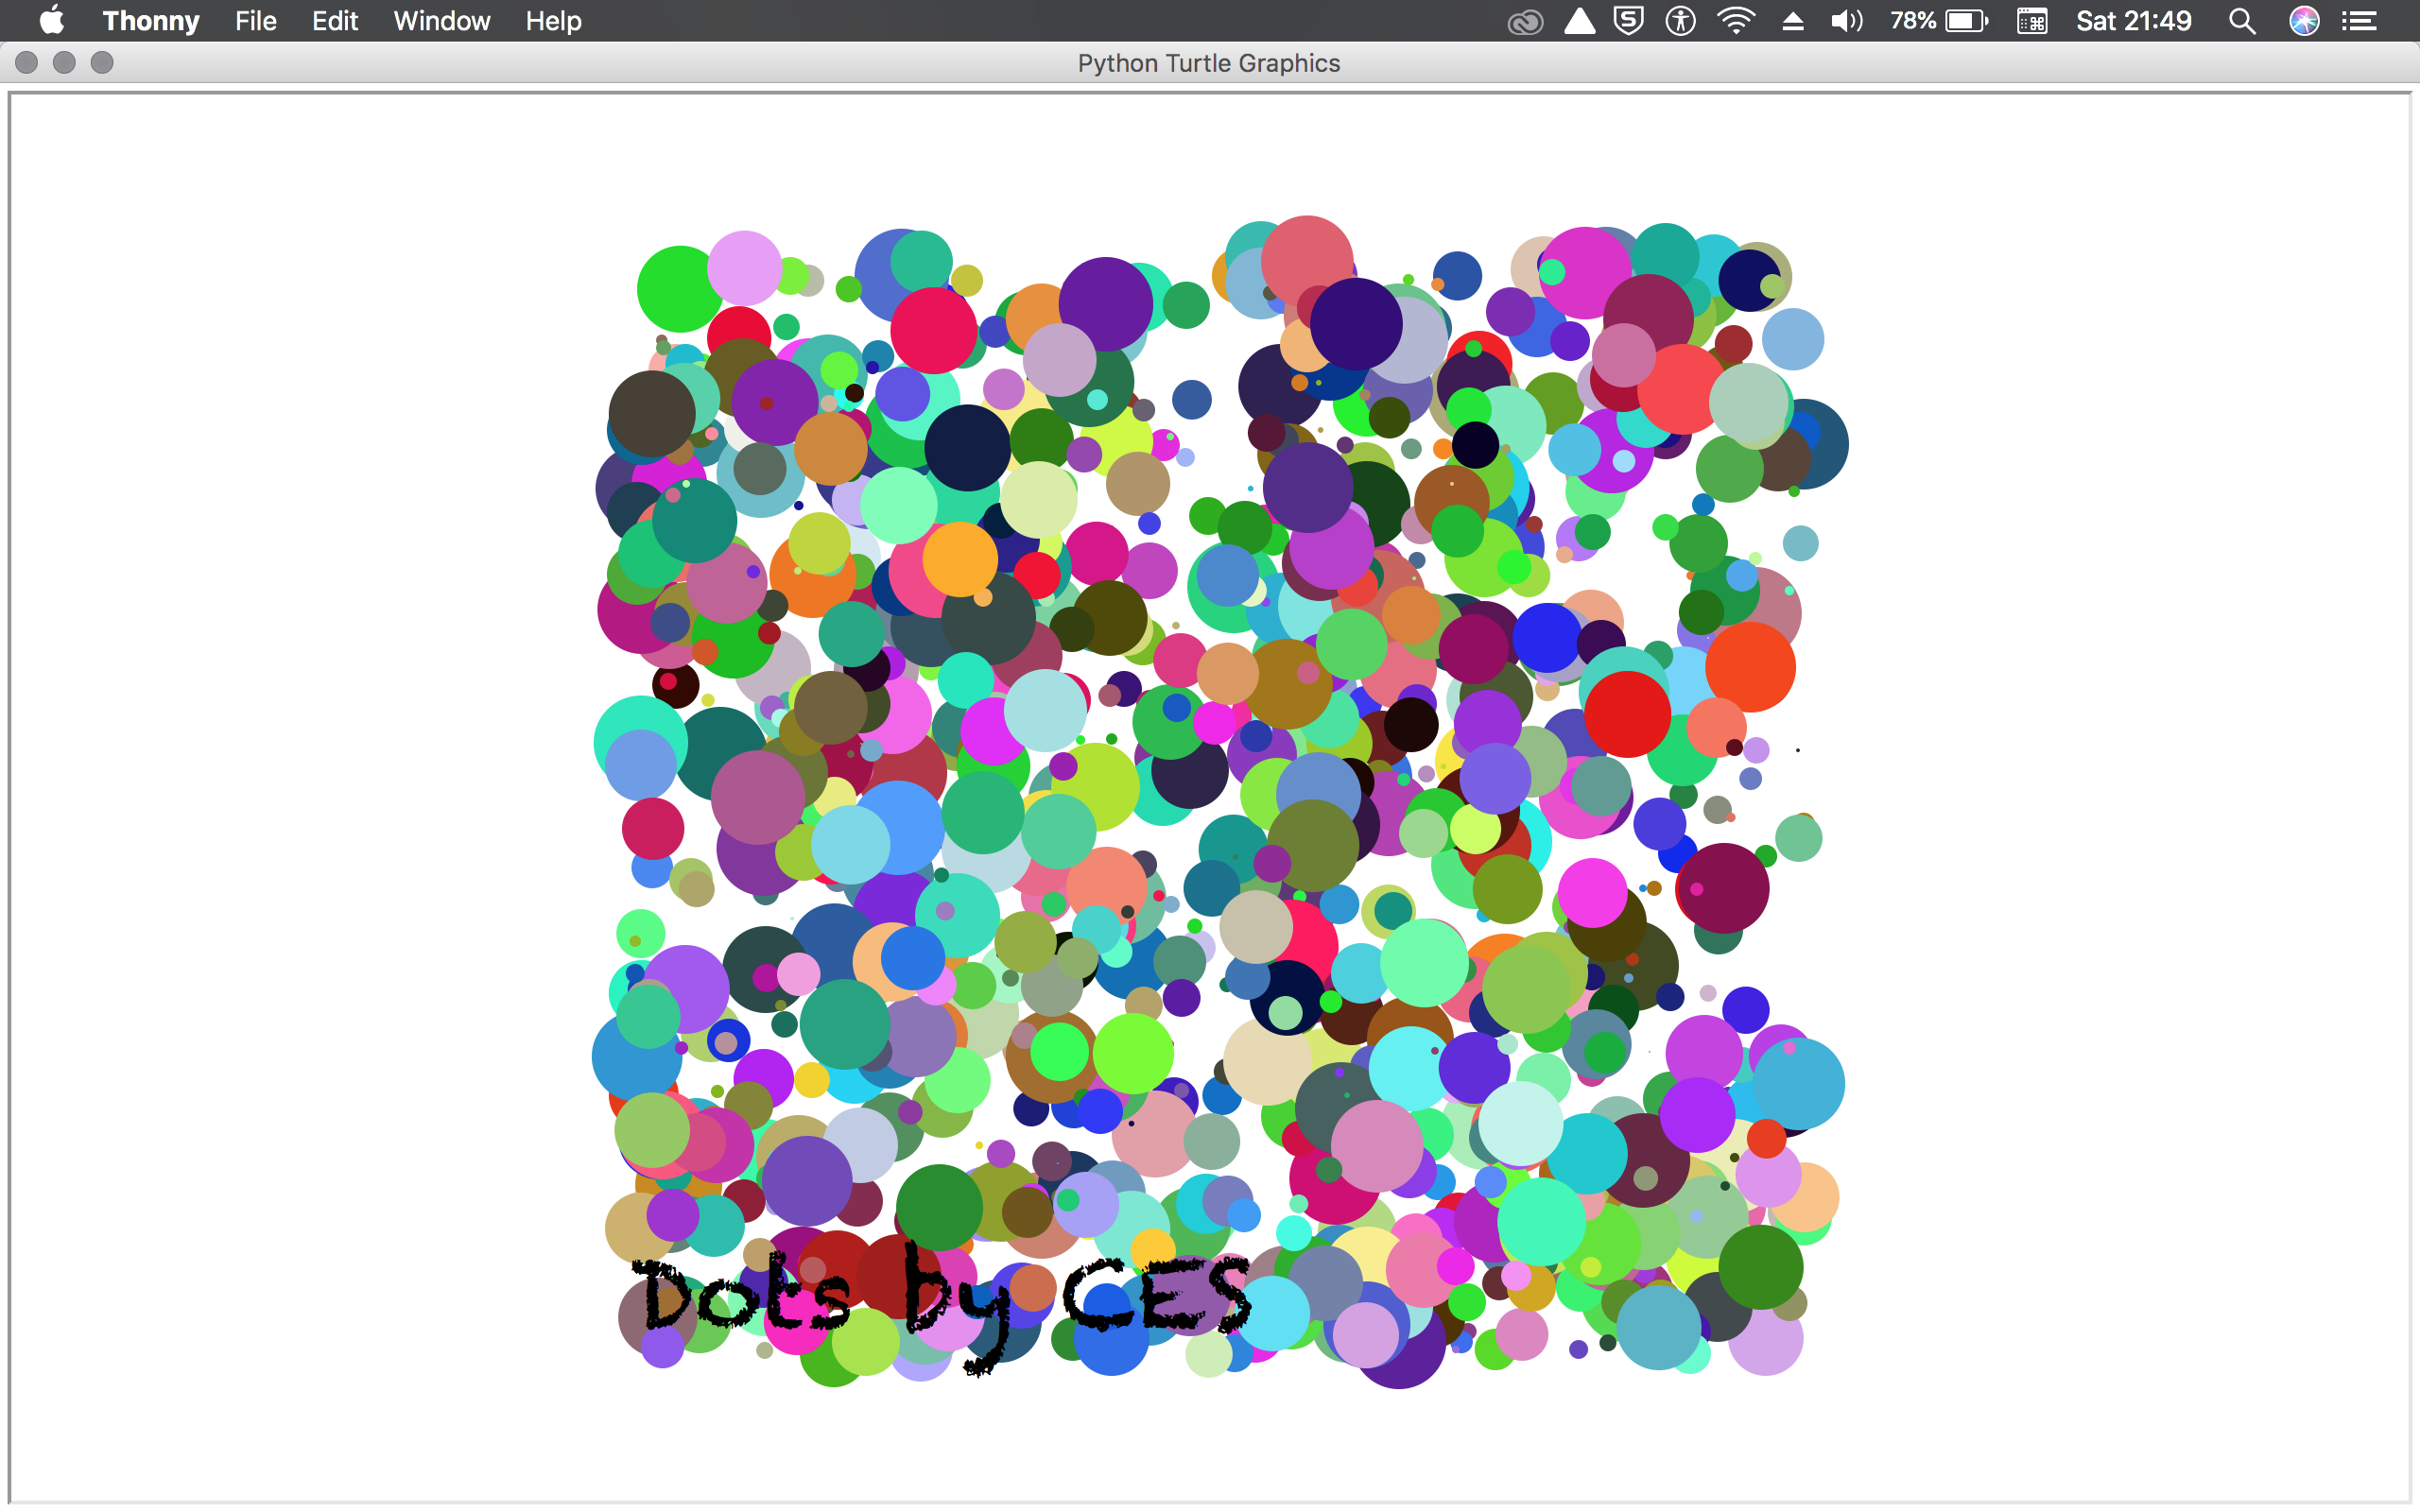
\includegraphics[width=\linewidth]{dots} %sample-franklin}
  \caption{1000 Dots, created with Turtle on Python v3. Randomized dot size, color, and location.}
  \Description{Turtle Art: Dots by CES}
\end{figure}

Your figures should contain a caption which describes the figure to
the reader. Figure captions go below the figure. Your figures should
{\bfseries also} include a description suitable for screen readers, to
assist the visually-challenged to better understand your work.

Figure captions are placed {\itshape below} the figure.

\subsection{The ``Teaser Figure''}

A ``teaser figure'' is an image, or set of images in one figure, that
are placed after all author and affiliation information, and before
the body of the article, spanning the page. If you wish to have such a
figure in your article, place the command immediately before the
\verb|\maketitle| command:
\begin{verbatim}
  \begin{teaserfigure}
    \includegraphics[width=\textwidth]{sampleteaser}
    \caption{figure caption}
    \Description{figure description}
  \end{teaserfigure}
\end{verbatim}



\section{Research Methods}

\subsection{Part One}

Lorem ipsum dolor sit amet, consectetur adipiscing elit. Morbi
malesuada, quam in pulvinar varius, metus nunc fermentum urna, id
sollicitudin purus odio sit amet enim. Aliquam ullamcorper eu ipsum
vel mollis. Curabitur quis dictum nisl. Phasellus vel semper risus, et
lacinia dolor. Integer ultricies commodo sem nec semper.

\subsection{Part Two}

Etiam commodo feugiat nisl pulvinar pellentesque. Etiam auctor sodales
ligula, non varius nibh pulvinar semper. Suspendisse nec lectus non
ipsum convallis congue hendrerit vitae sapien. Donec at laoreet
eros. Vivamus non purus placerat, scelerisque diam eu, cursus
ante. Etiam aliquam tortor auctor efficitur mattis.

\section{Online Resources}

Nam id fermentum dui. Suspendisse sagittis tortor a nulla mollis, in
pulvinar ex pretium. Sed interdum orci quis metus euismod, et sagittis
enim maximus. Vestibulum gravida massa ut felis suscipit
congue. Quisque mattis elit a risus ultrices commodo venenatis eget
dui. Etiam sagittis eleifend elementum.

Nam interdum magna at lectus dignissim, ac dignissim lorem
rhoncus. Maecenas eu arcu ac neque placerat aliquam. Nunc pulvinar
massa et mattis lacinia.

\end{document}
\endinput
%%
%% End of file `sample-manuscript.tex'.
